\section{Auswertung}
\label{sec:auswertung}

Die Fehlerrechnung übernimmt hier die Python-Bibliothek \texttt{uncertainties}.
Dieser liegt die Gauß'sche Fehlerfortpflanzung zugrunde:
\begin{equation*}
    \symup{\Delta} y = \sum_{i=1}^n \left| \frac{\delta f(x_1, \ldots, x_n)}{\delta x_i} \right| \symup{\Delta} x_i \ .
\end{equation*}


\subsection{Eichung des Magnetfelds} \label{sec:auswertung:eichung}
Um in den folgenden Auswertungsschritten
die jeweilige magnetische Flussdichte zu kennen,
wird zuerst eine Eichung des Elektromagneten durchgeführt,
wie in \autoref{sec:durchfuehrung} beschrieben.

Die entsprechenden Messwerte sind in \autoref{tab:eichung} angegeben
und in \autoref{fig:plt:eichung} grafisch dargestellt.

Mithilfe einer Regressionsrechnung unter Verwendung der Python-Bibliothek \texttt{numpy} % genauer: np.polyfit
ergeben sich für ein Polynom dritten Grades
\[
    B(I) = aI^3 + bI^2 + cI + d
\]
die Parameter
\begin{align*}
    a &= \SI{-0.45 \pm 0.04}{\milli\tesla\per\cubic\ampere} \\
    b &= \SI{-0.1 \pm 0.4}{\milli\tesla\per\square\ampere} \\
    c &= \SI{100.7 \pm 1.5}{\milli\tesla\per\ampere} \\
    d &= \SI{1.1 \pm 1.4}{\milli\tesla} \ .
\end{align*}

\begin{table}[H]
    \centering
    \caption{Magnetische Flussdichte in Abhängigkeit des Spulenstroms.}
    \label{tab:eichung}
    \begin{tabular}{S S}
        \toprule
        {$I \mathbin{/} \si{A}$} & {$B \mathbin{/} \si{\milli\tesla}$} \\
        \midrule
        0.0 &   6.0 \\
        0.2 &  23.6 \\
        0.4 &  41.8 \\
        0.6 &  59.6 \\
        0.8 &  80.0 \\
        1.0 &  99.4 \\
        1.2 & 117.8 \\
        1.4 & 138.3 \\
        1.6 & 157.1 \\
        1.8 & 178.0 \\
        2.0 & 198.4 \\
        2.2 & 217.7 \\
        2.4 & 236.1 \\
        2.6 & 254.9 \\
        2.8 & 273.6 \\
        3.0 & 292.0 \\
        3.2 & 307.8 \\
        3.4 & 324.9 \\
        3.6 & 343.0 \\
        3.8 & 361.2 \\
        4.0 & 375.5 \\
        4.2 & 392.5 \\
        4.4 & 406.8 \\
        4.6 & 421.3 \\
        4.8 & 434.8 \\
        5.0 & 448.5 \\
        5.2 & 460.2 \\
        5.4 & 473.2 \\
        5.6 & 484.9 \\
        5.8 & 495.6 \\
        6.0 & 506.3 \\
        6.2 & 514.9 \\
        6.4 & 522.9 \\
        6.6 & 530.7 \\
        6.8 & 538.3 \\
        7.0 & 546.5 \\
        7.2 & 553.3 \\
        7.4 & 559.0 \\
        7.6 & 570.5 \\
        7.8 & 575.8 \\
        8.0 & 575.5 \\
        \bottomrule
    \end{tabular}
\end{table}

\begin{figure}[H]
    \centering
    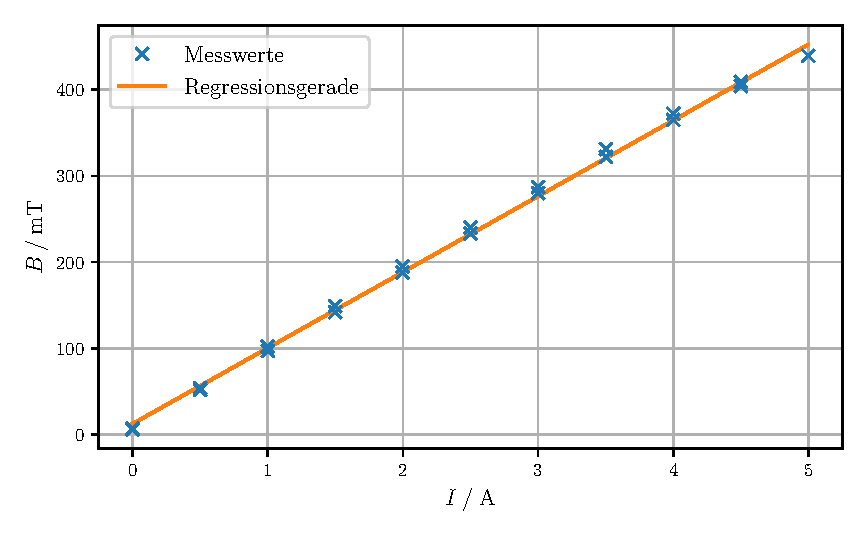
\includegraphics[width=\textwidth]{build/plt/1_magnet.pdf}
    \caption{Messwerte und Regressionspolynom zur Eichung des Elektromagneten.}
    \label{fig:plt:eichung}
\end{figure}

\subsection{Zur Umsetzung der Abstandsbestimmung von Spektrallinien}
Die Auswertung eines einzelnen Bilds erfolgt in den folgenden Schritten:
\begin{itemize}
    \item Die im Bild eingebettete Datumsangabe wird mit Schwarz übermalt, um die spätere Erkennung nicht zu stören.
          Dies ist problemlos möglich, da die Datumsangabe nur unwesentlich mit den Linien überlappt.
    \item Das Bild wird so rotiert, dass die einzelnen Linien möglichst vertikal ausgerichtet sind.
    \item Da davon auszugehen ist, dass das Bild keine verwertbaren Farbinformationen enthält, werden die RGB-Kanäle summiert.
    \item Für jede Pixel-Spalte wird eine Summe gebildet, sodass ein eindimensionales Array verbleibt,
          welches auf den Wertebereich $[0, 1]$ normiert wird.
    \item Mittels \href{https://docs.scipy.org/doc/scipy/reference/generated/scipy.signal.find_peaks.html}{\texttt{scipy.signal.find\_peaks}}
          und gegebenenfalls angepasster Suchparameter (\texttt{distance}, \texttt{height}, \texttt{prominence})
          werden die Maxima ermittelt,
          welche den Linien entsprechen, deren Abstand bestimmt werden soll.
    \item Da die Abstände in beliebigen Einheiten verwendet werden können,
          muss nur noch die Differenz der Indizes (und somit der Pixel) je zweier Maxima berechnet werden.
    \item Aus den einzelnen Abständen wird schließlich das arithmetische Mittel gebildet.
\end{itemize}

\subsection{Untersuchung der roten Spektrallinie}
Um den Landé-Faktor zum linear polarisierten roten Licht der Cadmium-Linie zu bestimmen,
wird der Abstand $\symup{\delta} s$ der Interferenzlinien ohne Magnetfeld
mit dem Abstand $\symup{\Delta} s$ der aufgespaltenen Interferenzlinien im Magnetfeld verglichen.
Diese Abstände werden in \autoref{tab:rot} aufgelistet.
\autoref{fig:plt:rot_1} und \autoref{fig:plt:rot_2} zeigen eine Überlagerung
aus den aufgenommenen Bildern und der durchgeführten Analyse.

Das zweite Bild wurde bei einem Spulenstrom von \SI{8}{\ampere} aufgenommen,
welcher nach \autoref{sec:auswertung:eichung} einer magnetischen Flussdichte von \SI{573.67 \pm 35.62}{\milli\tesla} entspricht.
% TODO: Polarisierung

Die gemittelten Werte lauten
\begin{align*}
    Δs &= \SI{247.8}{px} \\
    δs &= \SI{111.7}{px} \ .
\end{align*}

Es wird auf die Angabe einer Unsicherheit verzichtet,
da bekannt ist, dass diese Abstände von links nach rechts zunehmen \cite{versuchsanleitung},
weshalb der Fehler andernfalls überschätzt würde.


Das für die Wellenlänge $\lambda = \SI{643.8}{\nano\meter}$ nach \autoref{eqn:dispersionsgebiet} berechnete Dispersionsgebiet ist
\[
    \symup{\Delta}\lambda_\text{D} = \SI{48.913}{\pico\meter} \ .
\]

Die Aufspaltung
\begin{equation}
    \label{eqn:delta_lambda}
    \symup{\delta} \lambda = \frac{1}{2} \frac{\symup{\delta} s}{\symup{\Delta} s} \symup{\Delta} \lambda_\text{D}
\end{equation}
berechnet sich damit im Mittel zu
\[
    \symup{\delta} \lambda = \SI{11.021}{\pico\meter} \ .
\]

Mit
\begin{equation}
    \label{eqn:g_mess}
    g = \frac{hc \symup{\delta} \lambda}{\lambda^2 \mu_{\symup{B}} B}
\end{equation}
folgt
\[
    g = \num{0.99 \pm 0.06} \ .
\]


\begin{table}[H]
    \centering
    \caption{
        Pixelabstände $\symup{\Delta} s$ und $\symup{\delta} s$ bei aus- beziehungsweise eingeschaltetem Magnetfeld.
        Peaks sind durch rote Linien hervorgehoben.
    }
    \label{tab:rot}
    \begin{tabular}{S S S}
        \toprule
        {$I \mathbin{/} \si{\ampere}$} & 0 & 8 \\
        {$B \mathbin{/} \si{\milli\tesla}$} & 0 & 573.67 \pm 35.62 \\
        \midrule
        & {$\symup{\Delta} S$} & {$\symup{\delta} S$} \\
        \midrule
        \expandableinput{build/tab/rot.tex}
        \bottomrule
    \end{tabular}
\end{table}

\begin{figure}[H]
    \centering
    
\includegraphics[width=\textwidth]{build/plt/rot_1.pdf}
    \caption{Bild/Plot mitausgeschaltetem Elektromagneten.}
    \label{fig:plt:rot_1}
\end{figure}

\begin{figure}[H]
    \centering
    
\includegraphics[width=\textwidth]{build/plt/rot_2.pdf}
    \caption{Bild/Plot miteingeschaltetem Elektromagneten.}
    \label{fig:plt:rot_2}
\end{figure}


\FloatBarrier
\subsection{Untersuchung der blauen, sigma-polarisierten Spektrallinie} \label{sec:auswertung:blau_sigma}
Die Abstände $\symup{\delta} s$ und $\symup{\Delta} s$ werden analog zum Vorgehen bei der roten Spektrallinie
in \autoref{tab:blau_sigma} aufgelistet.
\autoref{fig:plt:blau_sigma_1} und \autoref{fig:plt:blau_sigma_2} zeigen eine Überlagerung
aus den aufgenommenen Bildern und der durchgeführten Analyse.

Das zweite Bild wurde bei einem Spulenstrom von \SI{4.6}{\ampere} aufgenommen,
welcher nach \autoref{sec:auswertung:eichung} einer magnetischen Flussdichte von \SI{419.45 \pm 12.13}{\milli\tesla} entspricht.
% TODO: Polarisierung

Die gemittelten Werte lauten
\begin{align*}
    Δs &= \SI{53.2}{px} \\
    δs &= \SI{23.2}{px} \ .
\end{align*}


Das für die Wellenlänge $\lambda = \SI{480.0}{\nano\meter}$ nach \autoref{eqn:dispersionsgebiet} berechnete Dispersionsgebiet ist
\[
    \symup{\Delta}\lambda_\text{D} = \SI{26.952}{\pico\meter} \ .
\]

Die Aufspaltung berechnet sich damit (wie zuvor gemäß \autoref{eqn:delta_lambda}) im Mittel zu
\[
    \symup{\delta} \lambda = \SI{5.877}{\pico\meter} \ .
\]

Mit \autoref{eqn:g_mess} folgt:
\[
    g = \num{1.30 \pm 0.04} \ .
\]

\begin{table}[H]
    \centering
    \caption{Pixelabstände $\symup{\Delta} s$ und $\symup{\delta} s$ bei aus- beziehungsweise eingeschaltetem Magnetfeld.}
    \label{tab:blau_sigma}
    \begin{tabular}{S S S}
        \toprule
        {$I \mathbin{/} \si{\ampere}$} & 0 & 4.6 \\
        {$B \mathbin{/} \si{\milli\tesla}$} & 0 & 419.45 \pm 12.13 \\
        \midrule
        & {$\symup{\Delta} S$} & {$\symup{\delta} S$} \\
        \midrule
        \expandableinput{build/tab/blau_sigma.tex}
        \bottomrule
    \end{tabular}
\end{table}

\begin{figure}[H]
    \centering
    
\includegraphics[width=\textwidth]{build/plt/blau_sigma_1.pdf}
    \caption{Bild/Plot mitausgeschaltetem Elektromagneten.}
    \label{fig:plt:blau_sigma_1}
\end{figure}

\begin{figure}[H]
    \centering
    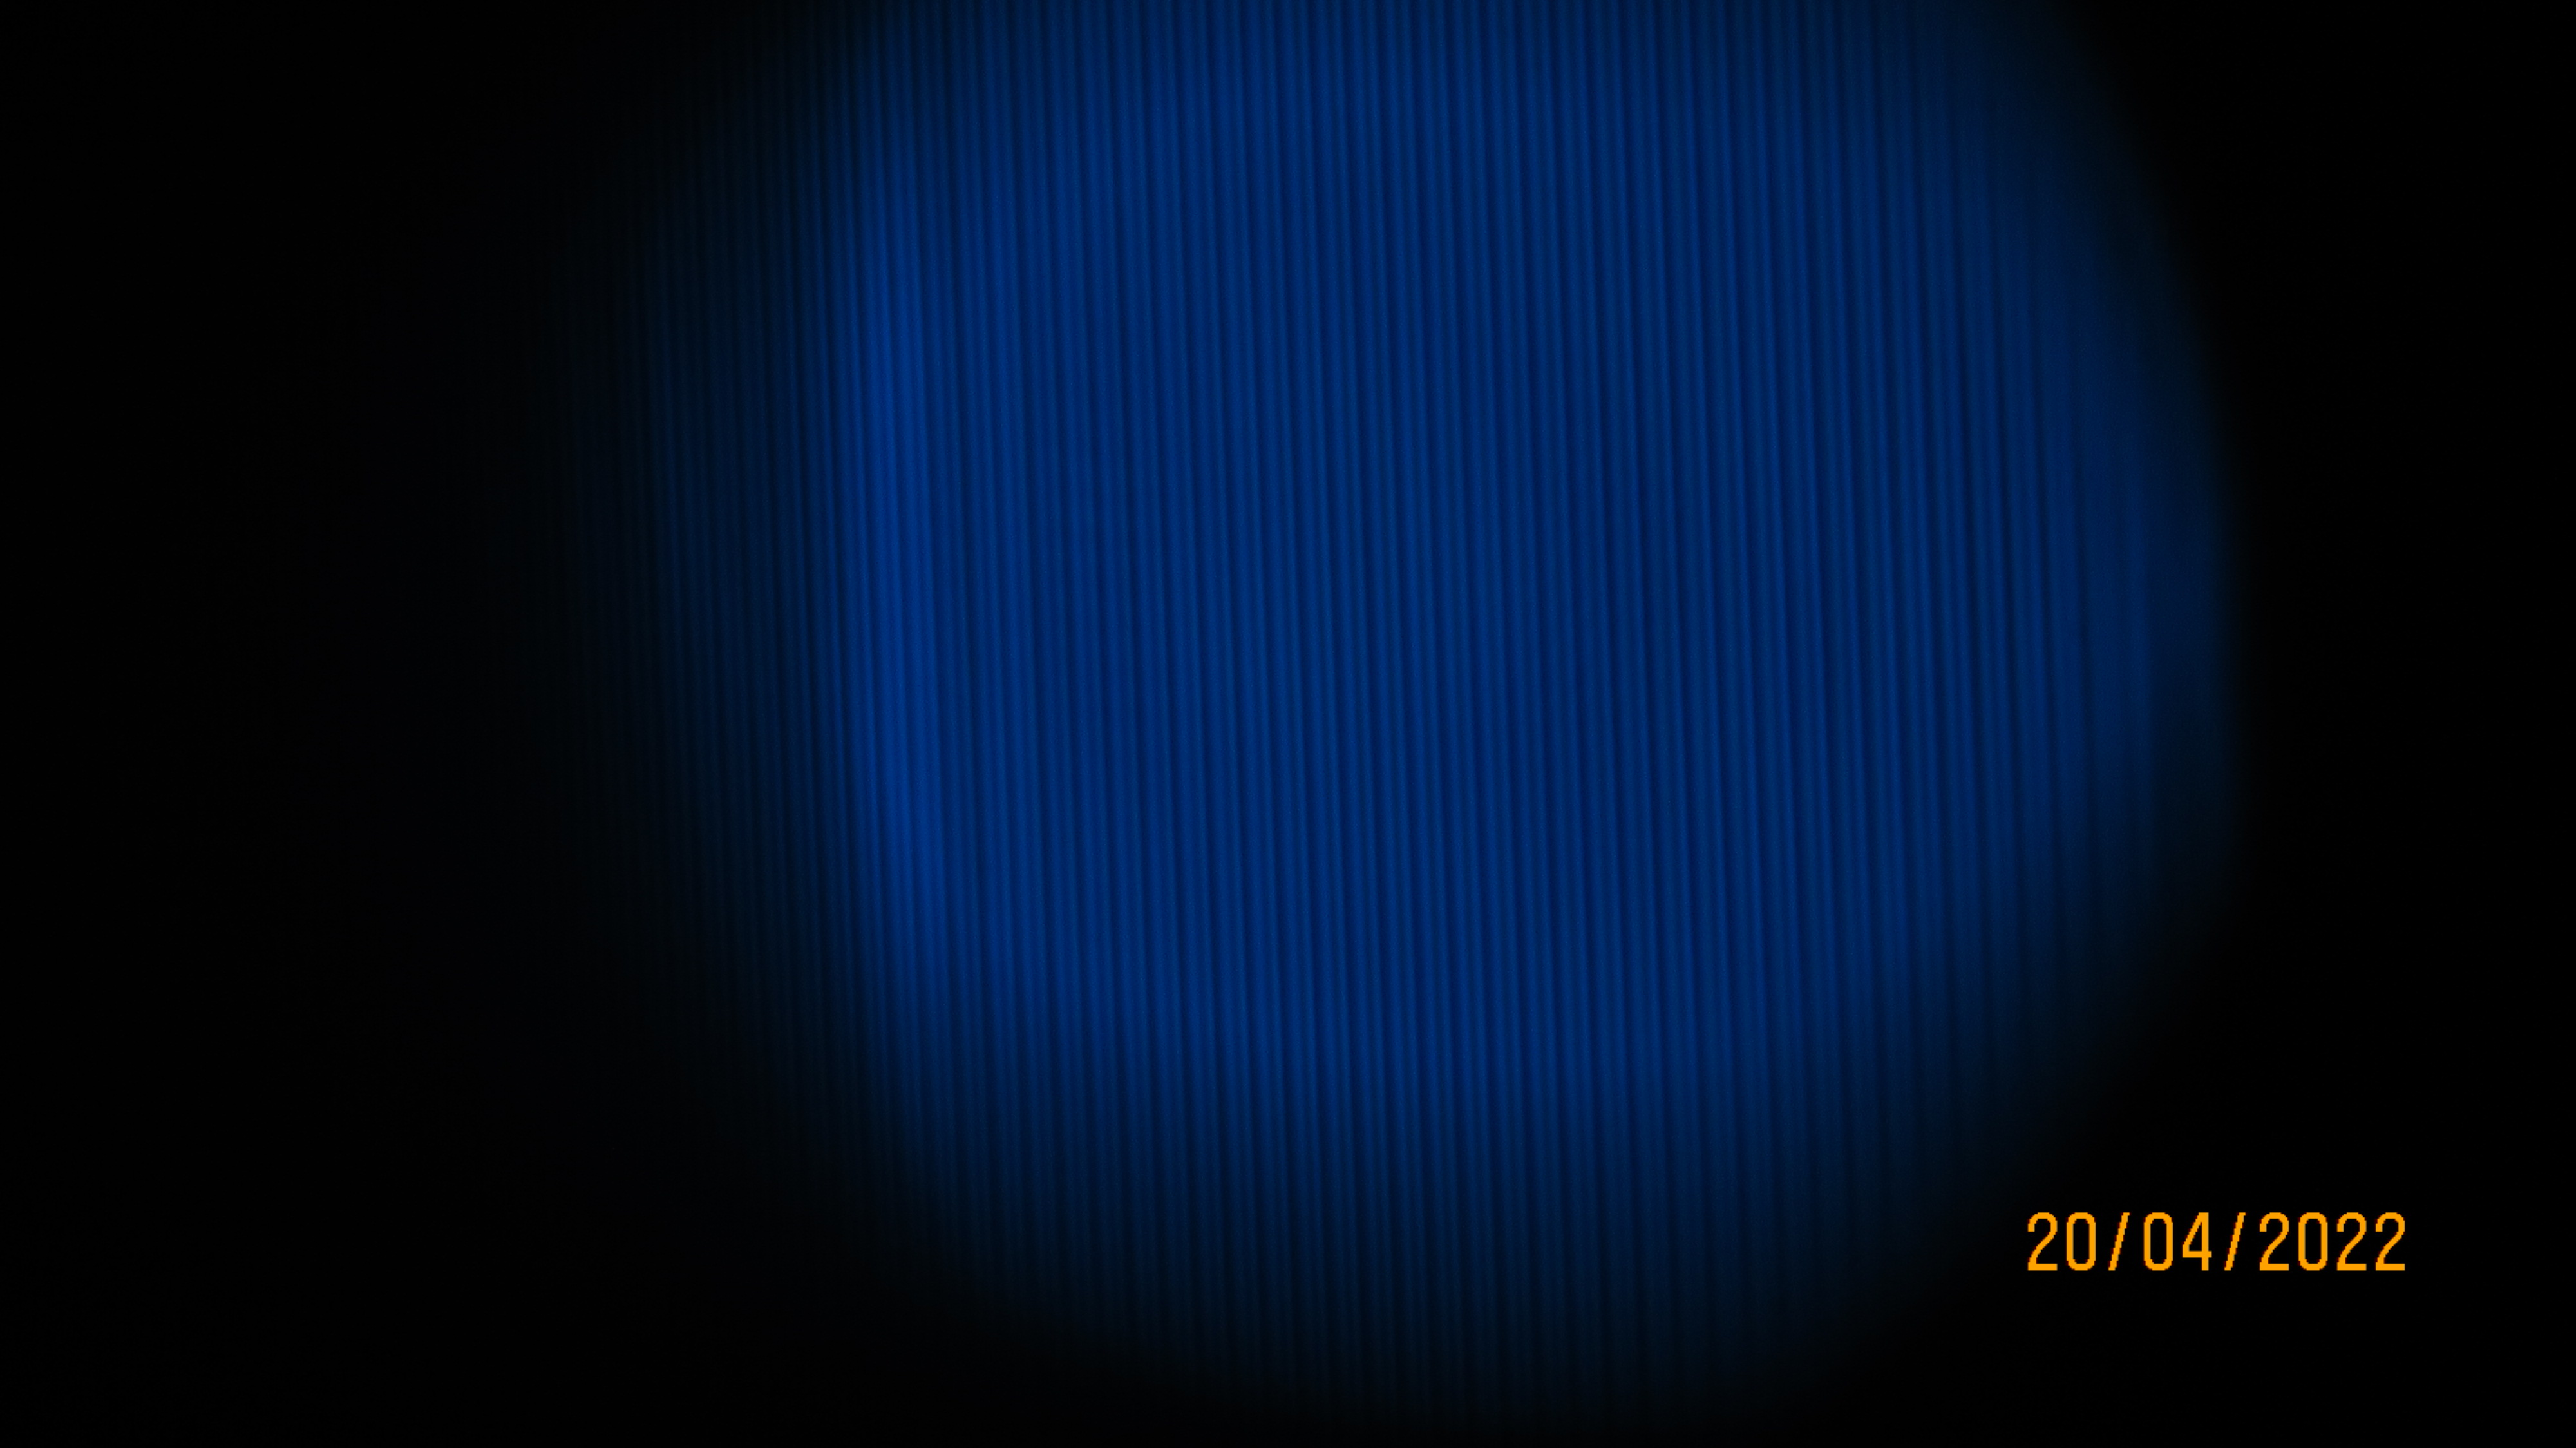
\includegraphics[width=\textwidth]{build/plt/blau_sigma_2.pdf}
    \caption{Bild/Plot miteingeschaltetem Elektromagneten.}
    \label{fig:plt:blau_sigma_2}
\end{figure}


\FloatBarrier
\subsection{Untersuchung der blauen, pi-polarisierten Spektrallinie}
Die Abstände $\symup{\delta} s$ und $\symup{\Delta} s$ werden analog zum Vorgehen bei der roten Spektrallinie
in \autoref{tab:blau_sigma} aufgelistet.
\autoref{fig:plt:blau_pi_1} und \autoref{fig:plt:blau_pi_2} zeigen eine Überlagerung
aus den aufgenommenen Bildern und der durchgeführten Analyse.

Das zweite Bild wurde bei einem Spulenstrom von \SI{8}{\ampere} aufgenommen,
welcher nach \autoref{sec:auswertung:eichung} einer magnetischen Flussdichte von \SI{573.67 \pm 35.62}{\milli\tesla} entspricht.
% TODO: Polarisierung

Die gemittelten Werte lauten
\begin{align*}
    Δs &= \SI{53.2}{px} \\
    δs &= \SI{23.2}{px} \ .
\end{align*}


Die Aufspaltung berechnet sich
mit demselben $\symup{\Delta}\lambda_\text{D}$ aus \autoref{auswertung:blau_sigma}
im Mittel zu
\[
    \symup{\delta} \lambda = \SI{6.101}{\pico\meter} \ .
\]

Mit \autoref{eqn:g_mess} folgt:
\[
    g = \num{0.99 \pm 0.06} \ .
\]

\begin{table}[H]
    \centering
    \caption{Pixelabstände $\symup{\Delta} s$ und $\symup{\delta} s$ bei aus- beziehungsweise eingeschaltetem Magnetfeld.}
    \label{tab:blau_pi}
    \begin{tabular}{S S S}
        \toprule
        {$I \mathbin{/} \si{\ampere}$} & 0 & 8 \\
        {$B \mathbin{/} \si{\milli\tesla}$} & 0 & 573.67 \pm 35.62 \\
        \midrule
        & {$\symup{\Delta} S$} & {$\symup{\delta} S$} \\
        \midrule
        \expandableinput{build/tab/blau_pi.tex}
        \bottomrule
    \end{tabular}
\end{table}

\begin{figure}[H]
    \centering
    
\includegraphics[width=\textwidth]{build/plt/blau_pi_1.pdf}
    \caption{Bild/Plot mitausgeschaltetem Elektromagneten.}
    \label{fig:plt:blau_pi_1}
\end{figure}

\begin{figure}[H]
    \centering
    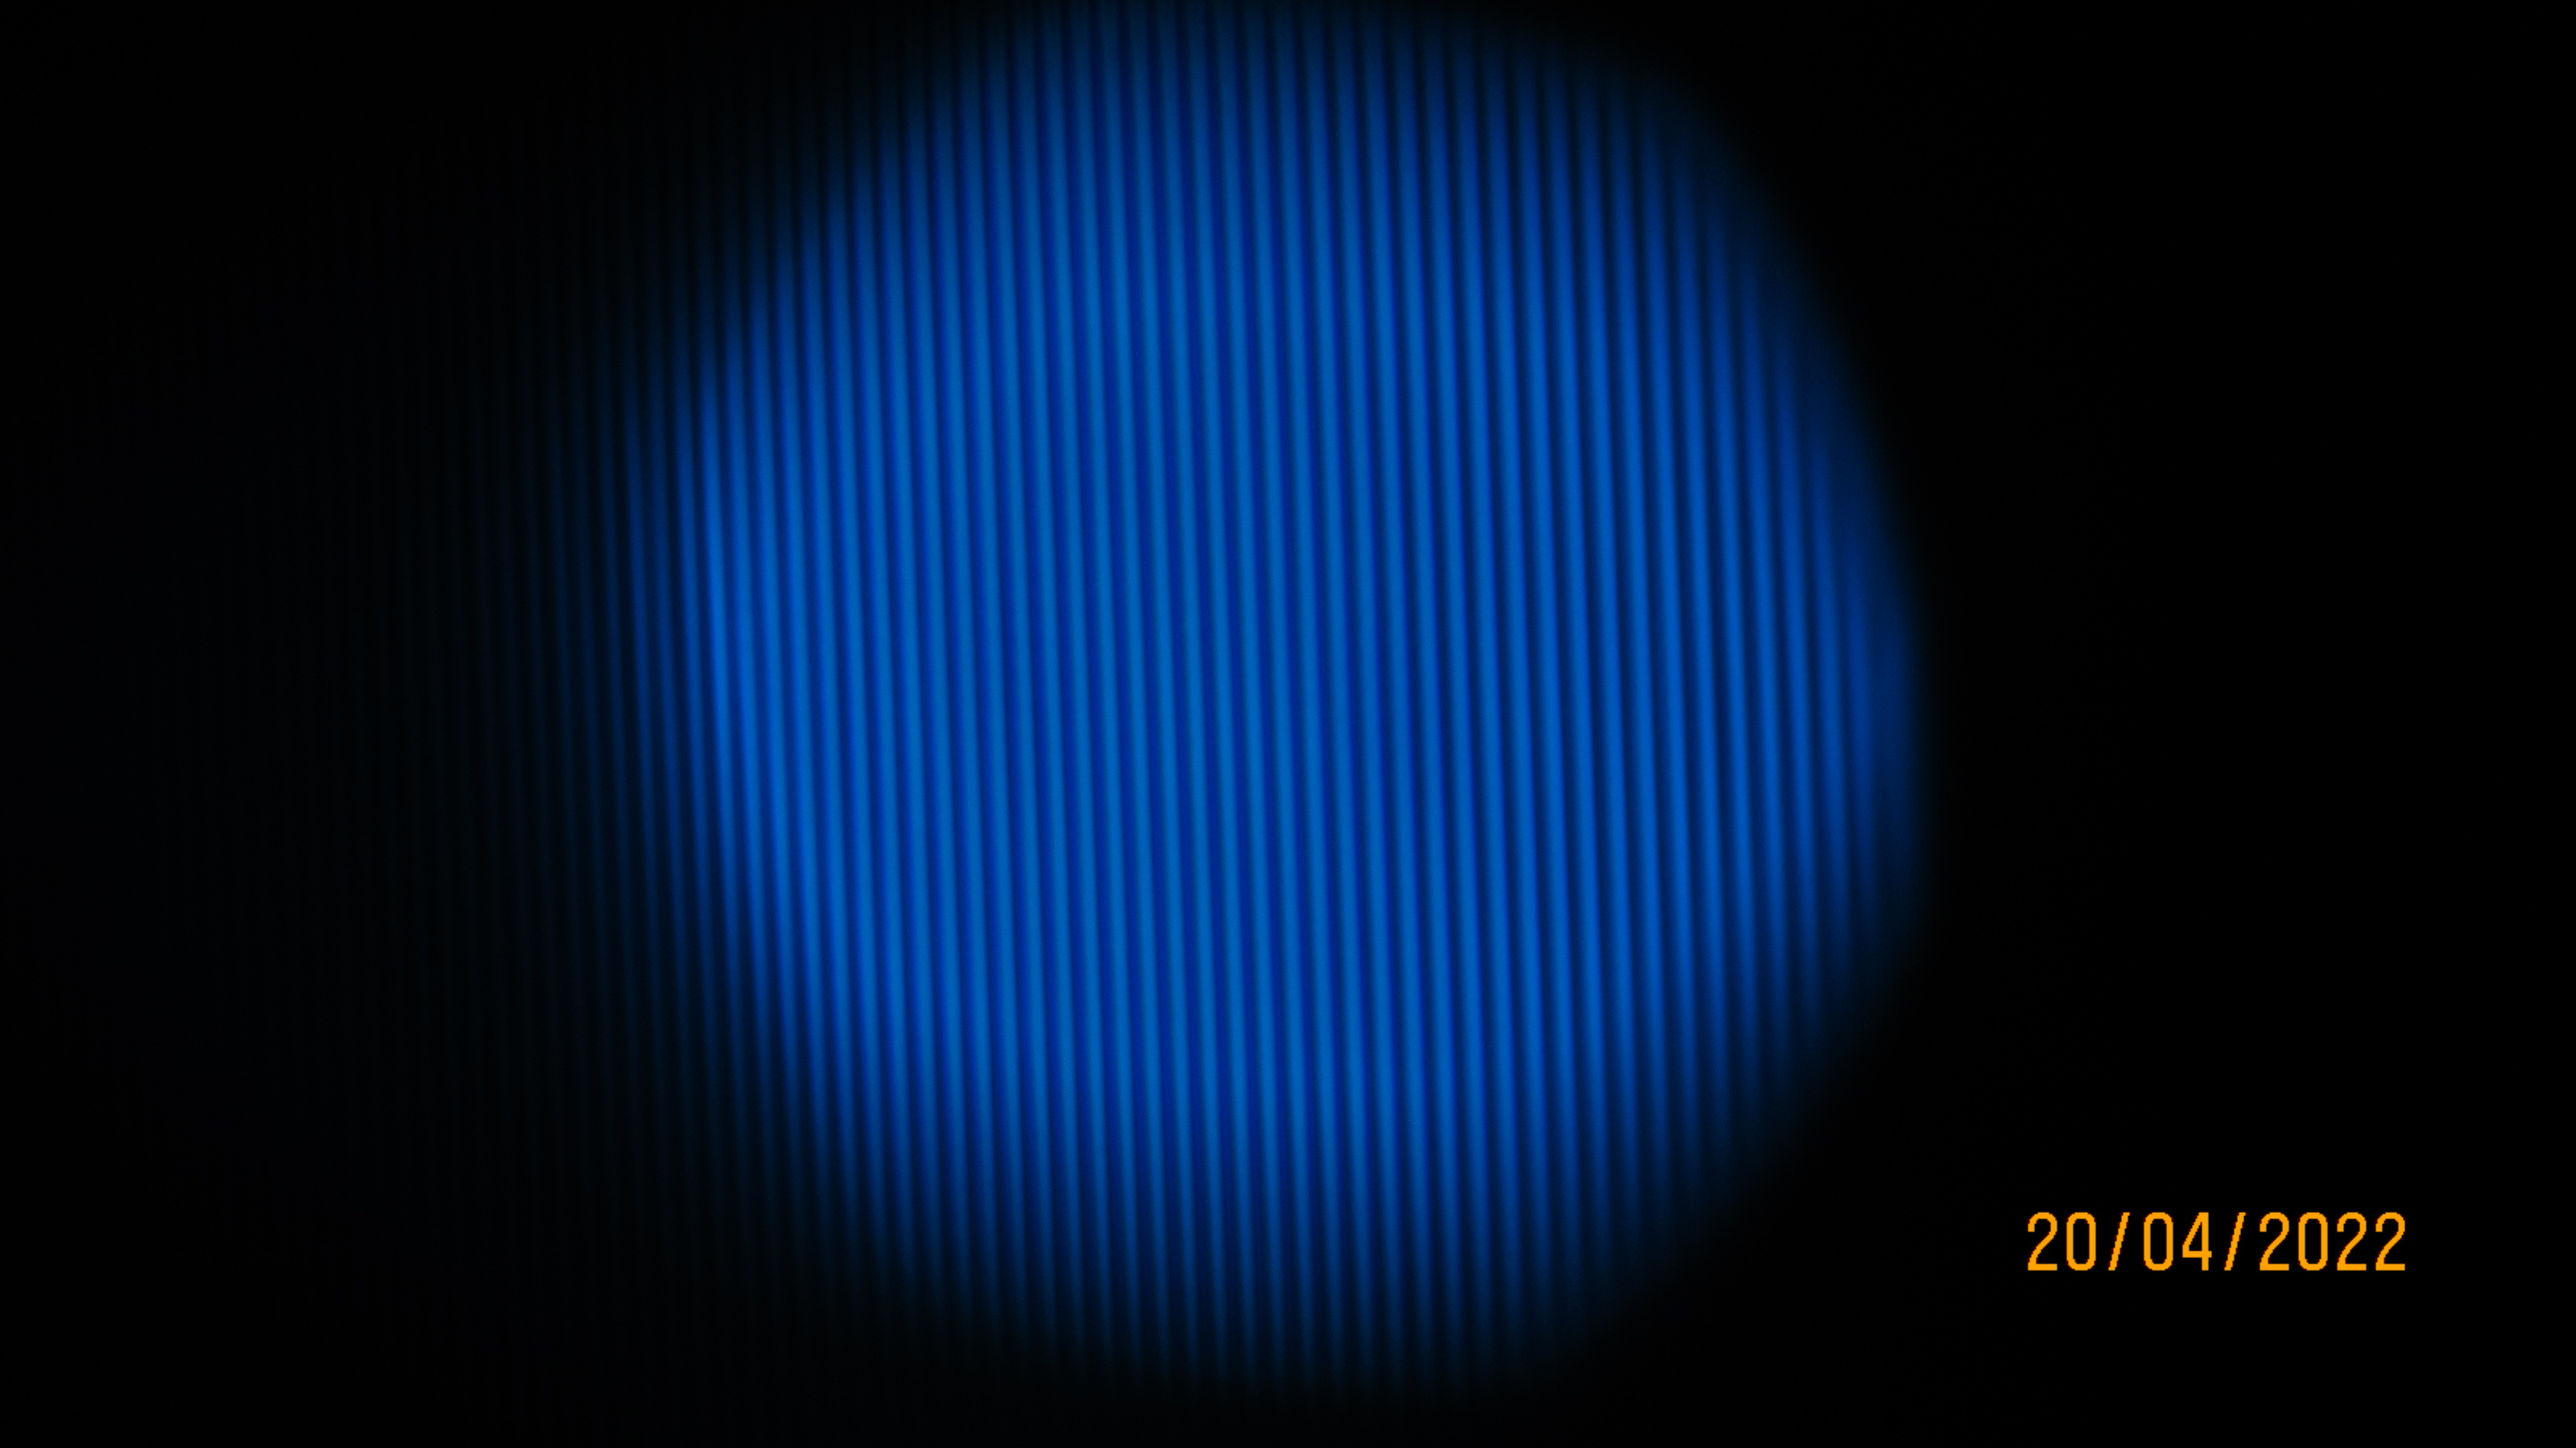
\includegraphics[width=\textwidth]{build/plt/blau_pi_2.pdf}
    \caption{Bild/Plot miteingeschaltetem Elektromagneten.}
    \label{fig:plt:blau_pi_2}
\end{figure}
